\documentclass{article} % This command is used to set the type of document you are working on such as an article, book, or presenation
\usepackage{amsmath}  % This package allows the use of a large range of mathematical formula, commands, and symbols=]
\usepackage[linguistics]{forest}
\usepackage{tikz}

\begin{document}

\title{multiFaAcceleration: A program for the measurement of mutation velocity and acceleration from a four-species multiple alignment}
\author{Riley J. Mangan}
\maketitle

\section{Usage}
multiFaAcceleration - Performs velocity and acceleration on a four way multiple alignment in multiFa format.\par
A four way multiple alignment must contain four species (index 0 to 3) in the topology that species 1 to 3 are successive outgroups of species 0.\par
While this program accepts an alignment of any four species in this configuration, this program was initially written for a multiple alignment of Human, Chimpanzee, Gorilla, and Orangutan. Variable names in this documentation and in the code itself are named according to these species names.\par
Three bed files are returned. The first produces the normalized velocity score, the second returns the normalized acceleration score, and the third returns the normalized initial velocity score for each window of the genome for aln[0] (Human). This program can also produce the raw Velocity and Initial Velocity branch lengths as optional returns.\par
multiFaAcceleration chromName in.fa velocity.bed acceleration.bed initialVelocity.bed\par

\section{Distance-based phylogenetic inference with the Fitch-Margoliash method}

Consider a phylogenetic tree with four extant species (Human, Chimpanzee, Gorilla, Orangutan), two extinct ancestors (Human-Chimp Ancestor (HCA) and Human-Gorilla Ancestor (HGA)), and branch lengths (BhumHca, BchimpHca, HCA-HGA, BhgaGor, BhgaOrang) with the following topology.\par

\begin{center}
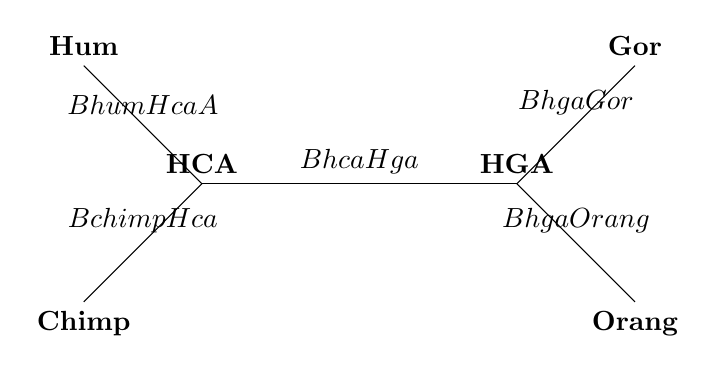
\begin{tikzpicture}
\node[above] at (-2,0) {$\textbf{HCA}$};
\draw (-2,0) -- node[above] {$BhcaHga$} (2,0) node[above] {$\textbf{HGA}$};
\draw (-2,0) -- node[above] {$BhumHcaA$}(-3.5,1.5) node[above] {$\textbf{Hum}$};
\draw (-2,0) -- node[above] {$BchimpHca$}(-3.5,-1.5) node[below] {$\textbf{Chimp}$};
\draw (2,0) -- node[above] {$BhgaGor$}(3.5,1.5) node[above] {$\textbf{Gor}$};
\draw (2,0) -- node[above] {$BhgaOrang$}(3.5,-1.5) node[below] {$\textbf{Orang}$};\
\end{tikzpicture}
\end{center}

Consider that we can measure the pairwise mutation distance between any two extant species on this tree, represented by $D_{ij}$. The distance defined by the sum of branch lengths, also known as the patristic distance, is represented as $d_{ij}$. It follows that the pairwise distance between two extant species is equal to the sum of branch lengths separating those species on the phylogenetic tree shown above. Thus, we are able to produce the following system of linear equations.

\begin{equation}
\begin{split}
&D_{hum-chimp} \approx d_{hum-chimp} =  BhumHca + BchimpHca\\
&D_{hum-gor} \approx d_{hum-gor} = BhumHca + BhcaHga + BhgaGor\\
&D_{chimp-gor} \approx d_{chimp-gor} = BchimpHca + BhcaHga + BhgaGor\\
&D_{hum-orang} \approx d_{hum-orang} = BhumHca + BhcaHga + BhgaOrang\\
&D_{chimp-orang} \approx d_{chimp-orang} = BchimpHca + BhcaHga + BhgaOrang\\
&D_{gor-orang} \approx d_{gor-orang} = BhgaGor + BhgaOrang
\end{split}
\end{equation}

If our interest is to study Human genome evolution, we can define the mutation distance as $BhumHca$, the distance between the human sequence and the sequence of its most recent ancestor with chimpanzees. We can then define the initial mutation distance as $BhcaHga$, the distance along the previous branch the inferred Human-Chimp ancestor and the common ancestor between humans and gorillas (HGA).\par
We can compute branch lengths using the method of Fitch and Margoliash \cite{pmid5334057} with an alternating least squares optimization algorithm developed by Felsenstein \cite{pmid11975348}. While the full details and derivations for these methods can be found in these two papers, I will briefly explain the method below.\par
Due to such phenomenon as back mutation and discrepancies in INDEL-sensitive distance metrics, it is not always possible to find a set of branch lengths for the above system of equations such that $D_{ij} = d_{ij} \: \forall \: i,j \in S$, where $S$ is the set of all extant species. Thus, in the Fitch-Margoliash method, we aim to find a set of branch lengths $B$ that minimizes the squared difference between the pairwise and patristic distances. In symbolic terms:
\begin{equation*}
	Q = \sum_{i \in S}\sum_{j \in S}w_{ij}(D_{ij} - d_{ij})^2
\end{equation*}
In the above expression, $w_{ij}$ represents a weight for error terms, and serves to place more of the overall error in the estimated branch lengths on longer branches. This expression is of the form:
\begin{equation*}
\begin{split}
	w_{ij} = \frac{1}{D_{ij}^2} \mid D_{ij} \ne 0\\
\end{split}
\end{equation*}

When $D_{ij} = 0$, the weight term $w_{ij}$ approaches positive infinity. In this program, we approximate this limit by assigning an arbitrarily large number to $w_{ij}$. This value is $1000$ by default, but can be controlled by the user with the option $zeroDistanceWeightConstant$.

\section{Tree reduction and subtree optimization}
In the alternating least squares approach top optimize Q described by Felsenstein, we must first reduce the above tree, which contains two internal nodes $HCA$ and $HGA$, to subtrees containing only one internal node. These subtrees, which we refer to as the left and right subtrees, are shown below.

Left subtree:
\begin{center}
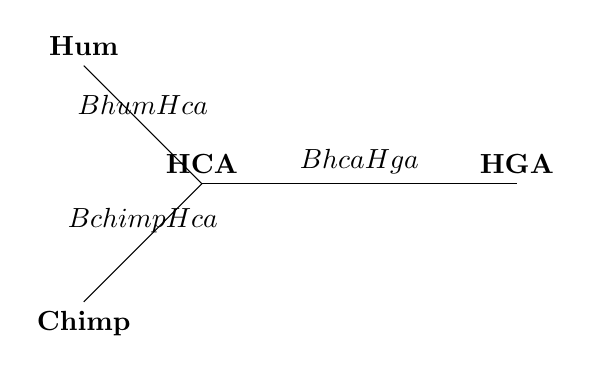
\begin{tikzpicture}
\node[above] at (-2,0) {$\textbf{HCA}$};
\draw (-2,0) -- node[above] {$BhcaHga$} (2,0) node[above] {$\textbf{HGA}$};
\draw (-2,0) -- node[above] {$BhumHca$}(-3.5,1.5) node[above] {$\textbf{Hum}$};
\draw (-2,0) -- node[above] {$BchimpHca$}(-3.5,-1.5) node[below] {$\textbf{Chimp}$};
\end{tikzpicture}
\end{center}

Right subtree:
\begin{center}
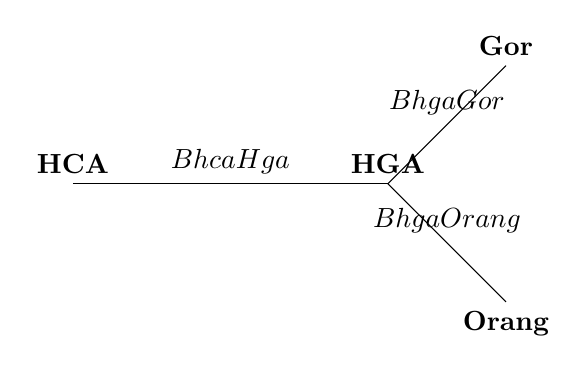
\begin{tikzpicture}
\node[above] at (-2,0) {$\textbf{HCA}$};
\draw (-2,0) -- node[above] {$BhcaHga$} (2,0) node[above] {$\textbf{HGA}$};
\draw (2,0) -- node[above] {$BhgaGor$}(3.5,1.5) node[above] {$\textbf{Gor}$};
\draw (2,0) -- node[above] {$BhgaOrang$}(3.5,-1.5) node[below] {$\textbf{Orang}$};\
\end{tikzpicture}
\end{center}

In the $multiFaAcceleration$ program, these subtrees are produced with the $pruneLeft$ and $pruneRight$ helper functions, respectively. To find the optimal branch lengths for these subtrees, we must find the pairwise distances between the extant species nodes and the ancestral node which is now a leaf in the subtree. For the left subtree, Felsenstein demonstrates that we can calculate these distances as:
\begin{equation*}
	D_{HumHga} = \frac{w_{HumGor}(D_{HumGor} - BhgaGor) + w_{Humorang}(D_{HumOrang} - BhgaOrang)}{w_{HumGor} + w_{HumOrang}}
\end{equation*}
\begin{equation*}
	D_{ChimpHga} = \frac{w_{ChimpGor}(D_{ChimpGor} - BhgaGor) + w_{ChimpOrang}(D_{ChimpOrang} - BhgaOrang)}{w_{ChimpGor} + w_{ChimpOrang}}
\end{equation*}
Similarly, for the right subtree:
\begin{equation*}
	D_{HcaGor} = \frac{w_{HumGor}(D_{HumGor} - BhgaGor) + w_{ChimpGor}(D_{ChimpGor} - BhgaOrang)}{w_{HumGor} + w_{ChimpGor}}
\end{equation*}
\begin{equation*}
	D_{HcaOrang} = \frac{w_{HumOrang}(D_{HumOrang} - BhgaGor) + w_{ChimpOrang}(D_{ChimpOrang} - BhgaOrang)}{w_{HumOrang} + w_{ChimpOrang}}
\end{equation*}
As distance is necessarily a non-negative quantity, and the weight constant is set to an arbitrarily large number when $D_{ij} = 0$, the denominator in the above equations can never be zero, and does not need to be otherwise constrained.\par
The three-species left subtree with branch lengths $v$ has the following optimal branch lengths:
\begin{equation*}
\begin{split}
v_a = \frac{(D_{ab} + D_{ac} - D_{bc})}{2}\\
v_b = \frac{(D_{ab} + D_{bc} - D_{ac})}{2}\\
v_c = \frac{(D_{ac} + D_{bc} - D_{ab})}{2}
\end{split}
\end{equation*}

\section{Constraint for non-negative branch lengths}
In some cases, the optimal set of branch lengths for the minimization of Q will include negative branch lengths. While this can be allowed by the user with the option $allowNegative$, this program constrains branch lengths to non-negative values by default. Briefly, when one or more branches from the 3-species subtrees are evaluated as negative values, they are set to 0. From Felsenstein 1997, if branch lengths $v_b$ or $v_c$ are set to zero in this fashion, the new optimal branch length for $v_a$, given that either of these terms are set to zero, can be approximated as:
\begin{equation*}
	\hat v_a = \frac{w_{ab}(D_{ab} - v_b) + w_{ac}(D_{ac} - v_c)}{w_{ab} + w_{ac}}
\end{equation*}

\section{Algorithm for branch length calculations}
With these equations in hand, we can now describe the algorithm for computing optimal branch lengths for the four-species tree, which is performed by the helper function $alternatingLeastSquares$ in $multiFaAcceleration$. First, the set of output branch lengths are initialized such that each branch length is equal to 1. In each iteration, the tree is first pruned to the left subtree, and the branch lengths $BhumHca, BchimpHca, BhcaHga$ are then set to the optimal branch lengths for this subtree. Next, the tree is pruned into the right subtree, and the branches $BhcaHga, BhgaGor, BhgaOrang$ are then set to the optimal values for this subtree. Once both optimizations have occurred, the value of Q is calculated for the current branch lengths and compared to the value of Q observed in the previous iteration. If the difference between the estimates of Q falls below a user-specified level of error $\epsilon$, the answer is returned. Otherwise, a new iteration is initiated. This heuristic will converge on a local minimum for Q and achieve stationarity in finite iterations. Due to the approximation used for non-negative branch lengths, it is possible stationarity will be achieved as the oscillation between two sets of branch lengths. In this case, we take the set of branch lengths associated with the lowest value of Q.
\section{Genome-wide acceleration calculation}
For a given four-way alignment in multiFa format, $gonomics:multiFaAcceleration$ calculates $BhumHca$ and $BhcaHga$ using pairwise mutation distance (defined as the number of SNPs and INDELs, where each INDEL counts as one mutation regardless of length) for each window of a user-specified window size. Windows may be every possible window of the genome, or may be restricted to a particular subset of the genome using the option $-searchSpaceBed$, which enables the input of a bed file which specifies the regions that should be considered. The option $-searchSpaceProportion$ enables the user to consider all windows in which at least a user-specified proportion of bases are within the searchSpace.

We define $\textbf{v}$ as the normalized mutation velocity, or the normalized rate of mutation over the branch $BhumHca$. To calculate $\textbf{v}$, we calculate the average $BhumHca$ length $E(BhumHca)$ across all windows. For each window:
\begin{equation*}
	\textbf{v} = \frac{BhumHca}{E(BhumHca)}
\end{equation*}

Similarly, the normalized initial rate of mutation, or the normalized rate of mutation over the branch $BhcaHga$, can be calculated as:
\begin{equation*}
	\textbf{v}_0 = \frac{BhcaHga}{E(BhcaHga)}
\end{equation*}
Where $e(BhcaHga)$ is the average value of $BhcaHga$ over all windows.\par
$\textbf{v}$ and $\textbf{v}_0$ have intuitive numerical interpretations. If $\textbf{v} = 1$ for a particular window, the mutation rate in the branch $BhumHca$ is equal to the chromosome-wide average mutation rate. $\textbf{v} = 2$ would be found in a region evolving twice as quickly, and $\textbf{v} = 0.5$ in a region evolving at half the average rate. The same interpretations apply for $\textbf{v}_0$, the rate of evolution along the branch $BhcaHga$.\par
Finally, we define the quantity $\textbf{a}$, for acceleration, as the normalized change in mutation rate between branches branches $BhumHca$ and $BhcaHga$:
\begin{equation*}
\textbf{a} = \textbf{v} - \textbf{v}_0
\end{equation*}

The quantity $\textbf{a}$ is equal to zero when the mutation rate along $BhumHca$ is equal to the mutation rate along $BhcaHga$. As both $\textbf{v}$ and $\textbf{v}_0$ are normalized, this holds true even if $BhumHca$ and $BhcaHga$ are not equal in absolute length, which will be the case when the extant species are not separated by equal amounts of evolutionary time (in the example here, the distance between humans and chimpanzees, about six million years, is nearly triple the 2.5 million years separating the Human-Chimp Ancestor from the Human-Gorilla Ancestor). Positive values for $\textbf{a}$ indicate accelerated regions, and negative values suggest regions under negative acceleration, in which a region evolved at a slower rate along $BhumHca$ than $BhcaHga$.

\bibliographystyle{genres}
\bibliography{multiFaRefs}
 
\end{document}
